% arara: pdflatex: { shell: yes }
\documentclass{article}
\usepackage[utf8]{inputenc}
\usepackage{array}
\usepackage{hyperref}
\usepackage{float}
\usepackage{graphicx}
\usepackage{tabularx} 
\bibliographystyle{apacite}

\hbadness=10000
\hfuzz=10000pt

\begin{document}

\title{Homework Assignment: TCP/IP, OSI, and Encapsulation}
\author{Erick Gonzalez Parada 178145}
\date{\today}

\maketitle

\section*{Part 1: TCP/IP vs. OSI Model Comparison (4 points)}

\subsection*{1. Fill in the following table comparing the OSI model and the TCP/IP model:}

\begin{table}[H]
\centering
\begin{tabularx}{\textwidth}{|l|l|X|}
\hline
\textbf{Layer (OSI Model)} & \textbf{Equivalent Layer (TCP/IP Model)} & \textbf{Main Function} \\
\hline
Application & Application & Handles user applications (e.g., web browsing) \\
\hline
Presentation & Application & Formats and encrypts data \cite{gfg1} \\
\hline
Session & Application & Manages communication sessions \cite{gfg1} \\
\hline
Transport & Transport & Ensures reliable data transfer \cite{gfg2} \\
\hline
Network & Internet & Routes packets across networks \cite{gfg2} \\
\hline
Data Link & Network Access & Handles MAC addressing and framing \cite{fcc} \\
\hline
Physical & Network Access & Defines hardware transmission \cite{fcc} \\
\hline
\end{tabularx}
\end{table}

The information for this table was retrieved from the following image:

\begin{figure}[H]
	\centering
	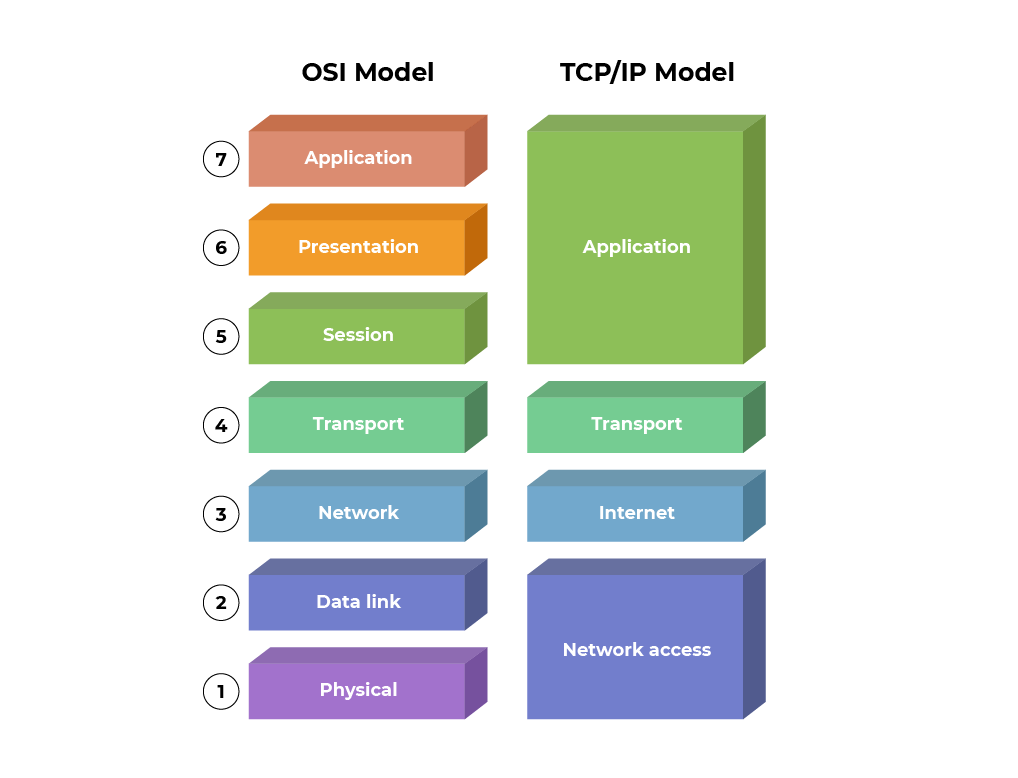
\includegraphics[width=1\textwidth]{tcpModel.png}
	\caption{TCP/IP Model vs. OSI Model}
	\label{fig:1}
\end{figure}

---

\section*{Part 2: Encapsulation Process (3 points)}

\subsection*{3. Arrange the following terms in order of encapsulation (from application to physical layer):}

The correct order of encapsulation is:
\begin{itemize}
    \item \textbf{Data} → \textbf{TCP Segment} → \textbf{IP Packet} → \textbf{Frame} → \textbf{Bits}
\end{itemize}

\subsubsection*{Explanation of Each Step:}
\begin{itemize}
    \item \textbf{Data}: The original message or payload created at the Application layer \cite{gfg1}.
    \item \textbf{TCP Segment}: At the Transport layer, the data is encapsulated into a TCP segment, which includes a header with information such as source and destination ports, sequence numbers, and checksums for reliable communication \cite{gfg2}.
    \item \textbf{IP Packet}: At the Network layer, the TCP segment is encapsulated into an IP packet, which adds a header containing source and destination IP addresses for routing across networks \cite{gfg2}.
    \item \textbf{Frame}: At the Data Link layer, the IP packet is encapsulated into a frame, which includes a header with MAC addresses for local network delivery and a trailer for error checking \cite{fcc}.
    \item \textbf{Bits}: At the Physical layer, the frame is converted into bits (binary 1s and 0s) for transmission over the physical medium (e.g., Ethernet cables or wireless signals) \cite{fcc}.
\end{itemize}

\subsection*{4. When sending a message over the Internet, at which layer does IP addressing occur?}
\begin{itemize}
    \item \textbf{C) Network} \cite{gfg2}
\end{itemize}

\subsection*{5. In de-encapsulation, which layer removes MAC addresses before sending data to the Network layer?}
\begin{itemize}
    \item \textbf{B) Data Link} \cite{fcc}
\end{itemize}

---

\section*{Part 3: Practical Scenario (3 points)}

\subsection*{6. Read the scenario below and answer the questions.}

\subsubsection*{Scenario:}
Alice is using a web browser to visit \texttt{www.example.com}. Her computer is connected to a router via Ethernet, and the website is hosted on a remote server.

\subsubsection*{Questions:}

\begin{itemize}
    \item \textbf{At which OSI layer does the HTTP request occur?}  
    \textbf{Answer:} The HTTP request occurs at the Application layer. This is where web browsers and web servers interact using the HTTP protocol to request and deliver web pages \cite{gfg1}.
    
    \item \textbf{Which protocol at the Transport layer will likely be used for this connection?}  
    \textbf{Answer:} The protocol used at the Transport layer will likely be TCP. TCP is commonly used for web traffic because it provides reliable, ordered, and error-checked delivery of data between applications \cite{gfg2}.
    
    \item \textbf{What happens to Alice's data at the Data Link layer before it is sent through Ethernet?}  
    \textbf{Answer:} At the Data Link layer, Alice's data is encapsulated into frames. The Data Link layer adds a header containing the source and destination MAC addresses, which are used for frame forwarding within the Local Area Network (LAN). The frame also includes a trailer for error detection (e.g., a CRC checksum). Once the frame is ready, it is sent through the Ethernet interface for transmission over the physical network \cite{fcc}.
\end{itemize}

---

\section*{References}

\begin{thebibliography}{9}
	\bibitem{gfg1}
	Improve, G. (2017a, August 30). \textit{What is OSI Model}. GeeksforGeeks. \\ 
	\url{https://www.geeksforgeeks.org/open-systems-interconnection-model-osi/}

	\bibitem{gfg2}
	Improve, G. (2017b, October 4). \textit{TCP/IP model}. GeeksforGeeks. \\ 
	\url{https://www.geeksforgeeks.org/tcp-ip-model/}

	\bibitem{fcc}
	Rosenbaum, O. (2022, October 21). \textit{How the Ethernet protocol works – A complete guide}. Freecodecamp.org. \\ 
	\url{https://www.freecodecamp.org/news/the-complete-guide-to-the-ethernet-protocol/}
\end{thebibliography}

\end{document}
